\renewcommand{\ttdefault}{pxtt}
\graphicspath{{chap2/figures/}}
\lstdefinelanguage{boogie}{%
  keywords={%
    procedure,var,int,call,return,assert,
  },
  morecomment=[l]{//},
}
\lstdefinelanguage{llvm}{%
  keywords={%
    define,void,alloca,call,bitcast,store,align,to,load,ret,void,getelementptr,icmp,
    inbounds,eq,
  },
  morecomment=[l]{//},
}

\lstdefinelanguage{rust}{%
  keywords={%
    fn,i1,i8,u8,i16,u16,i32,u32,i64,u64,mut,for,in,as,match,struct,let,mod,use,
    pub,extern,unsafe,bool
  },
  morecomment=[l]{//},
}


\newcommand{\lstrust}[1]{\lstset{language=C}\lstinline?#1?}
\newcommand{\lstllvm}[1]{\lstset{language=llvm}\lstinline?#1?}
\newcommand{\lstboogie}[1]{\lstset{language=boogie}\lstinline?#1?}
\newcommand{\rustc}{{rustc}}

\chapter[Verifying Rust Programs with SMACK]{Verifying Rust Programs\\ with SMACK\protect\footnotemark} \footnotetext{Adapted from \textit{Verifying Rust Programs with SMACK}, ATVA 2018~\cite{2018_atva_bhr}. Reproduced with permission from Springer Nature.}
\label{cha2}
\setupuuchapterbib
% \chapter{Verifying Rust Programs with SMACK}

%\author{Marek Baranowski \and Shaobo He \and Zvonimir Rakamari\'c}
%\institute{
%  School of Computing, University of Utah, USA \\
%  \email{\{baranows,shaobo,zvonimir\}@cs.utah.edu}
%}

%\begin{abstract}
%
Rust is an emerging systems programming language with guaranteed memory safety
and modern language features that has been extensively adopted to build
safety-critical software.
%
However, there is currently a lack of automated software verifiers for Rust.
%
In this work, we present our experience extending the SMACK verifier to enable
its usage on Rust programs.
%
We evaluate SMACK on a set of Rust programs to demonstrate a wide spectrum of
language features it supports.
%
\end{abstract}


\vspace{-2.5em}

\section{Introduction}
\label{sec:introduction}
Rust~\cite{rust-link,rust14} is a new programming language that aims
at enabling safe systems programming by means of an elaborate type
system.
%
It avoids memory safety issues prevalent in programs written in other
low-level programming languages such as C/C++ without adding performance
overhead often imposed by runtime systems or garbage
collectors.
%
Because of these merits, Rust has received a lot of attention from both
academia and industry, and it has been used to write production code shortly
after the release of version 1.0 in 2015.
%
Many industrial-strength safety-critical applications are being built in Rust,
such as web browsers, cloud storage, and embedded software~\cite{rust-friends,Levy2017}.


Although memory safety is enforced through type checking of
Rust programs at compile time, functional correctness (e.g., no violations of
user-specified assertions) is not guaranteed.
%
Automated software verifiers (e.g.,~\cite{smack-cav,ClarkeKL04,esbmc,calysto,cascade,Beyer2011,framac,gravy,tacas2007-clqr,joogie,klee,llbmc,satabs,symbc,tass,Albarghouthi2012,vcc,seahorn,civl})
based on
satisfiability modulo theories (SMT) solvers~\cite{smtlib} are a popular choice
for assuring the absence of assertion violations.
%
However, building a verifier, or extending an existing one, for a new language
is often tedious and time-consuming (e.g., implement a front-end, understand
and encode the language semantics).
%
For example, CRUST~\cite{crust}, a prototype verifier targeting memory safety
bugs in unsafe Rust code~\cite{unsafe-rust}, transforms Rust into C, which
makes it highly dependent on the still-evolving language details.
%
CRUST requires constant updates to keep up with the changes to Rust, which is a
large undertaking, and CRUST is no longer maintained.
%
To the best of our knowledge, currently there are no full-fledged, up-to-date
SMT-based verifiers for Rust.


In this chapter, we describe how we enable the verification of Rust
programs in the SMACK verifier~\cite{smack-cav,smack-web} with considerably less
effort than previous work~\cite{crust}.
%
Form more information about SMACK, please see \cref{sec:smackground}.
%
An advantage of SMACK is that it is input-language agnostic as it works by
verifying an intermediate representation (IR), specifically LLVM
IR~\cite{lattner2004llvm}.
%
Since the official Rust compiler, \rustc{}, can produce LLVM IR code corresponding
to Rust programs, a large front-end development effort was not needed as a rich
set of LLVM IR features is already supported by SMACK.
%any programming language with a compiler capable of emitting LLVM IR code can
%leverage SMACK's existing modeling of LLVM IR programs. Since Rust's official
%compiler, rustc, emits LLVM IR, it is natural to extend SMACK to support
%verification for programs written in this language.
%Even though C is currently the primary language that SMACK verifies, its input language agnosticism as a result of operating on an intermediate code representation (LLVM IR [4]) ostensibly allows the verification of any programming language with a compiler capable of pro- ducing LLVM IR, which is the case for Rust
%
%Nevertheless, extending SMACK to accept Rust programs is not push-button.
%
Rust is an emerging programming language that implements advanced language
features such as traits, smart pointers, and closures.
%
Hence, Rust's compiler emits LLVM IR code patterns that are often significantly
different from what is generated by the C compiler Clang~\cite{clang}, which is
the language that SMACK has primarily been used for.
%
Nevertheless, we managed to extend SMACK to support the verification of a
modern programming language such as Rust at a relatively small cost, and our
evaluation shows that it can already handle a variety of key language features.



%the focus of this paper is to present the missing
%components for extending SMACK to support Rust and interesting, novel
%augmentations done to SMACK during the extension.\shaobo{Talk about
%experiment results.}

% Should be a list 
%We will discuss the changes made to SMACK:
%\begin{itemize}
%  \item Changes made to enable SMACK to verify LLVM IR generated by
%the Rust compler.
%  \item Describe libraries that were developed to enable verification
%of non-trivial codes.
%  \item The development of a library to enable verification constructs
%to be expressed in idiomatic Rust.
%\end{itemize} Finally, we describe experiments which demonstrate real
%Rust programs which have been verified with the extended SMACK.




% \section{SMACK Software Verification Toolchain}
% \label{sec:background}
% 
\begin{figure}[tb]
  \centering
  \includegraphics[width=0.99\textwidth]{RustSmack}
  \caption{Toolflow of SMACK.}
  \label{fig:atvatoolflow}
\end{figure}

SMACK~\cite{smack14,smack} is a software verification toolchain that translates
LLVM IR code into Boogie intermediate verification language~\cite{boogie},
which is in turn verified using back-end Boogie verifiers such as
Corral~\cite{corral}.
%
Before our Rust effort, SMACK had been predominantly used to verify LLVM IR
programs produced by the Clang C compiler.
%
\Cref{fig:atvatoolflow} shows the toolflow of SMACK, which works as follows:
%
\begin{enumerate}
\item The SMACK top-level script automates the entire toolflow. It
  determines which compiler to invoke and flags to use for
  program compilation. In the case of C programs, it invokes Clang
  to generate LLVM IR code, while including SMACK's C language models.
  The models specify the semantics of common C library functions
  such as malloc, free, and string operations.
\item The common models file is then linked with the generated LLVM IR file to
  provide basic verification capabilities. This includes
  modeling dynamic memory allocation, supporting assertions and
  assumptions, and generating nondeterministic values.
\item The core \textsc{llvm2bpl} component takes an LLVM IR file as input, and
  produces Boogie code that captures the semantics of LLVM IR instructions;
  it outputs a Boogie file for verification.
\item Finally, the Corral back-end verifier is invoked on the generated Boogie
  file, and it uses Z3~\cite{z3} as its SMT solver. (Note that SMACK supports
  other back-end verifiers, which we omitted here.)
\end{enumerate}
%
In this work, we use Corral in its bounded verification mode, meaning that it
unrolls loops and recursion up to a certain user-provided bound.




\section{Rust-Driven Extensions to SMACK}
\label{sec:extensions}

\lstset{numbers=left,xleftmargin=2.5em}


%\zvon{Replace SmackVec with just Vec in the example. SmackVec will
%be confusing.} 
% Done
% \zvon{Change the font of the source code to match the one in this
% paper: http://soarlab.org/publications/cav2014-re.pdf. I think I
% did something when I moved the figure that changed its font.
% I don't like its current font.}
% Done

% \zvon{In this paragraph describe all interesting features of the
% example that are supported by SMACK. Refer to them in the example
% using line numbers. Do not hard-code them, but use labels, like
% I did with nondet below.}
% \zvon{Also say that we can do verification of programs that
% combine Rust and C.}
% Done and done.
\Cref{fig:crossfib} gives a Rust program illustrating
the language features that our SMACK extensions leverage or support.
%
%The Rust program on the left employs the vector library to implement the
%Fibonacci function using dynamic programming (lines
%\ref{code:fib_start}--\ref{code:fib_end}) and checks the equivalence between
%the Rust implementation \texttt{fib} and the C implementation \texttt{fib\_c}
%on the right.
%
Rust's foreign function interface (FFI) allows zero-cost interaction
with C code, verification of which had already been extensively supported by
SMACK.
%
As a result, we are able to reuse SMACK's C models as well as perform
cross-language verification of Rust programs containing calls to
external C functions (\cref{code:ffi}).
%
For example, we implemented macros \texttt{assume} (\cref{code:assume}) and \texttt{assert}
(\cref{code:assert}) to expand into calls to SMACK's built-in C functions.
%
\
\Cref{code:nondet} invokes the \lstrust{nondet} function that introduces
nondeterministic unconstrained values.
%
Note that we implemented these so that programs can be easily compiled into
executables even with SMACK annotations present --- in that case \lstrust{nondet}
is replaced with value \lstrust{5} in the example.


Instead of being undefined or triggering wrap-around behaviors as in C,
integer overflows in Rust are checked and can lead to \emph{program panic}.
%
For example, while not visible at the source level, the signed integer addition
operation at \cref{code:overflow} may optionally be checked for integer
overflows via the Rust compiler emitting LLVM arithmetic with overflow
intrinsics~\cite{llvm-intrinsics}; we had to extend SMACK to support such
intrinsics.
%
Finally, unlike C, standard libraries and modern language constructs such as the
\texttt{Vec} library (\cref{code:mkvec}) and iterators (\cref{code:iterator}) are abundant in Rust
code.
%
Modeling these libraries and language constructs is challenging yet essential
to build a practical Rust verifier; SMACK's modeling mechanism allowed us
to implement models for common Rust libraries.
%
We describe some of these extensions in more detail next.

%The \texttt{nondet()} method invoked in
%\cref{code:nondet} produces an arbitrary value when the program is
%verified by SMACK, but the concrete value 5 is used when compiled by
%\texttt{rustc}. Further, the \texttt{assume} macro
%(\cref{code:assume}) places constraints on what values the variable
%\texttt{n} may take, and the \texttt{assert} macro calls
%(\cref{code:assert}) SMACK's built-in assert function, these become an
%empty statement and Rust's built-in assert respectively when compiled
%with \texttt{rustc}. \Cref{code:mkvec} shows the creation of our
%modeled \texttt{Vec} class using a convenience macro of length
%\texttt{n+1}, and \cref{code:vectoridx} shows indexed assignment to
%the vector. Finally, \cref{code:ffi} invokes the C program's
%\texttt{fib\_c} function in order the two implementations. While not
%visible at the source level, \cref{code:overflow} may optionally be
%checked for overflow.



%% Rust provides a foreign function interface (FFI) which allows for
%% external function declarations with a syntax similar to C function
%% declarations. It is relatively simple to call these functions by
%% wrapping the function call in an {\tt unsafe} block. This allows us to
%% include SMACK's {\tt assert, assume} and {\tt nondet} functions in a
%% Rust program with relative ease. Rust considers locally defined macros
%% before other macros, allowing us to override the {\tt assert!} macro
%% to call SMACK's assert function. We implemented other macros such as
%% {\tt assume!} and {\tt nondet!} to constrain variables and produce
%% nondeterministic values respectively. Types in Rust are also flexible
%% in that new methods can be added to existing types through a type
%% trait. This allows us to implement a {\tt nondet} method for the
%% integer types in Rust. We combined the above features with Rust's
%% configuration system to allow Rust programs to transparently use SMACK
%% related extensions. For example, the statement \lstrust{let a = 7i32.nondet();}
%% will set \lstrust{a} to 7 when compiled normally, but \lstrust{a} will
%% have a nondeterministic value when the program is checked in SMACK.



% For Rust, the SMACK frontend invokes rustc to generate the LLVM IR.


%\subsection{Modifying the SMACK Toolflow}
%\label{sec:pipeline}
%
%In order to begin our investigation into integrating support for Rust
%programs in SMACK we had to make basic transformations to some parts
%of the LLVM IR code. These are:
%\begin{itemize}
%\item The \texttt{main} function generated by \rustc{} first calls a
%setup function before calling the program's true \texttt{main}
%function. We transformed the main function to call the
%real \texttt{main} function directly.
%\item Rust handles errors by invoking the \texttt{panic} function. The behavior
%of this function is to unwind the stack, similar to the way exceptions
%are handled in C++. However, Rust defines a panic as unrecoverable and
%terminates the program after it is invoked. We tranform panic calls
%into assertion failures with an annotation which indicates the program
%panicked.
%\item The Rust compiler emits the LLVM intrinsic \lstllvm{llvm.expect} which
%is an optimization hint. We modified SMACK to effectively tranform a call
%to this function to do nothing.
%\end{itemize}


\subsection{Supporting Rust-Generated LLVM IR Constructs}
\label{sec:llvm}


The LLVM IR code that \rustc{} emits contains several key constructs that are not
used in IR code produced by Clang.
%
Hence, we had to extend SMACK to add support for such constructs.
%
The Rust extensions to are highlighted by the dashed bordered boxes in \cref{fig:atvatoolflow}.

\subsubsection{Error Handling}
Rust handles errors by invoking the \texttt{panic} function. The behavior
of this function is to unwind the stack, similar to the way exceptions
are handled in C++. However, Rust defines a panic as unrecoverable and
terminates the program after it is invoked. We transform panic calls
into assertion failures with an annotation indicating the program
panicked.

% i1 and struct return
\subsubsection{Types}
%
The Rust compiler generates load/store instructions of the LLVM
\lstllvm{i1} data type, which is almost never emitted by Clang.
%
We added support for such instructions by zero-extending their operands to
\lstllvm{i8} when a store operation occurs, and casting them back when they are
loaded.
%
%This works for both the integer and bit-vector modes of Boogie.
%

Instructions operating on LLVM structure types occur frequently in
rustc-generated IR code, while Clang-generated IR almost always uses only
primitive types.
%
For example, it is a common practice for Rust programmers to use the
\lstrust{Option} type as the return type of functions.
%
It is generic over type \lstllvm{T} and represented in LLVM IR as
structure type \lstllvm{\{T,i1\}}, where setting \lstllvm{i1} is used to
indicate a valid return value.
%
%Hence, returning LLVM structures from functions is common in the LLVM
%IR code of Rust programs.
%
Moreover, load/store instructions over structures are frequently generated by
rustc, but not by Clang.
%
Hence, SMACK did not have an elaborate support for such instructions.


We support such instructions by modeling LLVM structure types using
uninterpreted functions that constrain each field.
%
For example, value \lstllvm{\{v,1\}} of type \lstllvm{\{T,i1\}} is
represented using an integer \lstboogie{s} with constraint \lstboogie{f(s,0)==v
&& f(s,1)==1}, where \lstboogie{f} is an uninterpreted function with the second
argument being the index of a structure field.
%
Such encoding allows us to model two basic LLVM structure instructions
\lstllvm{extractvalue} and \lstllvm{insertvalue} that read and write structure
fields, respectively.
%
Loads and stores of structures into memory are recursively translated into a sequence of
instructions that generate load/store for each field of primitive type, in conjunction with
the two aforementioned instructions.
%
%We extended SMACK to handle such constructs by first recursively flattening
%the
%structure type into a sequence of primitive types.
%
%Then, we extend the function signature with ``out parameters'' capturing
%the flattened structure.
%
%Finally, we instrument function returns so that the return values
%are extracted from a structure and placed into the out parameters;
%we also instrument function calls to read from the out parameters
%and store the read values into the respective structure.
%
This extension enables SMACK to handle structure constructs without
us having to introduce extensive modifications to its underlying memory model.

\subsubsection{Integer Packing}
%
The Rust compiler frequently packs smaller structures into 8-byte integers.
%
For example, rustc optimizes loading of a structure of type \lstllvm{\{i32,i32\}} into
loading of \lstllvm{i64}.
%
This requires less scalable bit-precise reasoning to be selected in
SMACK to avoid false bugs~\cite{aplas2017}.
%
Hence, we added an analysis pass to SMACK that detects load/store
instructions with pointer operands of integer element type that refer to
structures.
%
We translate such instructions to load/store directly from/into structure fields
(following the encoding described earlier),
thereby essentially avoiding packing.
%
This approach helps to scale the verification of Rust programs by avoiding the
need for bit-precise reasoning.

\subsubsection{Intrinsics}
%
We added support for two types of LLVM intrinsics heavily used by \rustc{}:
\lstllvm{llvm.expect} and arithmetic with overflow.
%
The Rust compiler emits the LLVM intrinsic \lstllvm{llvm.expect} as an
optimization hint. We modified SMACK to transform a call to this intrinsic into
essentially a no-op.
%
As future work, we will explore leveraging such hints to speed up
verification.


\lstset{numbers=left,xleftmargin=1.9em}


The Rust compiler typically emits instructions for checking all integer
operations for overflow through the use of LLVM arithmetic with overflow
intrinsics, such as \lstboogie{llvm.uadd} \lstboogie{.with.overflow.i32}.
%
The intrinsics indicate the sign and bitwidth in which to perform the given
operation.
%
We extended SMACK with an integer overflow checking pass that replaces
the intrinsics with instruction sequences implementing
the corresponding overflow checking.
%
\Cref{fig:overflow} shows an example translation:
\begin{itemize}
%\item On line 1, we first remove the checked overflow intrinsic.
\item Lines 2 and 3 extend the precision of the arguments to double the original bitwidth,
thereby avoiding potential overflow.
\item Line 4 computes the result of the addition, while line 5 converts the result
back to the original bitwidth.
\item Line 6 determines whether the operation overflowed, while line 7 checks it.
\end{itemize}
%
Note that the translation shown in \Cref{fig:overflow} is not optimal for dynamic checking since we optimized it for SMT-based verification with SMACK.
%
Furthermore, while the conversion of the intrinsic is always performed, checking is made optional following the convention that it is disabled in the release mode.
%% The overflow instructions indicate the signed-ness of
%% the operands, so we can always find the correct bounds for the
%% operation given the sign, e.g., \lstllvm{uadd} versus \lstllvm{sadd},
%% and the given bitwidth. If we do not consider overflow to be an
%% error, then we skip the result comparison and set \lstboogie{\$flag :=
%% true;}



\subsection{Modeling Rust Libraries}

Standard Rust libraries define most of the language's containers as generic
over the contained type, and generate the corresponding code for the
container when the program is compiled.
However, the generated code is heavily optimized for performance,
and contains constructs and functions that are difficult for
SMACK to analyze, such as custom allocators.
Hence, we leveraged SMACK's existing modeling capabilities to
write models for popular Rust data structures, such as vector (\lstrust{Vec}).
Vector is a dynamically-sized array used in many Rust programs as well as
for implementing other data structures such
as stacks and queues.
%
Currently, our vector model supports dynamic resizing, push, pop, get and
mutable get, and indexing among other features.
%
The model resides in a separate file, which SMACK automatically links as a Rust
module.


%\texttt{smack.rs} includes function declarations for SMACK's raw verification
%functions through Rust's foreign function intefrace (FFI). This file
%constitutes the ``Rust models'' component and provides access to these
%functions through macros (e.g., \lstrust{assert!}
%and \lstrust{assume!}) and convenience methods implemented to
%introduce nondeterministic integers through the \lstrust{nondet}
%method. Of note, the model file is written to be compiled
%conditionally, allowing for Rust programs to be compiled normally with
%SMACK annotations present.


\section{Experiments}
\label{sec:experiments}

We developed a benchmark suite containing various Rust language features
to test the SMACK extensions we developed.
\cref{tab:benchmarks} summarizes our benchmark suite.
Every category includes both correct and buggy benchmark versions.
Some notable included features are as follows:
\begin{itemize}
\item The closures category creates a closure that is passes to
  another function.
\item The generics category implements a generic trait for two
  generic structures.  A statically dispatched function is then
  invoked on the structures.
\item The vector category tests dynamic resizing and indexing
  of the Rust vector.
\item The cross-language category contains Rust
  programs that invoke C functions, including the \Cref{fig:crossfib} benchmark.
\item The ifc category contains the \textit{information
  flow control} (IFC) example from related \\ work~\cite{rust-safety17}. IFC models an
  access control method where access authority can only be
  increased. Using nondeterministic access levels, we verify that the
  IFC Rust implementation only allows access to the appropriate
  authority.
\end{itemize}
%
Currently, SMACK verifies most benchmarks in under 20 minutes.
The only exception is the full-blown IFC benchmark version that takes
several hours to complete.
%
The development of the benchmark suite helped us to identify
key language features that SMACK struggled with, and hence it guided our
efforts.
%
We plan to make our benchmark suite publicly available to bootstrap
the development of Rust verifiers.



\section{Limitations and Future Work}
\label{sec:future}
While the described extensions we made to SMACK enable its usage on many Rust
programs, some work remains.
%
First, SMACK currently does not precisely model virtual function tables
generated by a pointer to a structure which implements a trait (i.e., dynamic
polymorphism).
%
We will work towards supporting virtual function tables.
%
Second, Rust programs extensively rely on its standard libraries.
%
While we implemented models for the most common ones, such as \texttt{Vec}, we
plan to model a more substantial subset in the future.
%
% many of the function calls made by Rust
%libraries, e.g., those made by the \texttt{Vec} class, are opaque to SMACK.
%This necessitates the modeling of Rust's libraries rather than relying on
%their definitions. By changing the memory functions used in the Rust libraries
%and a MIR plugin, SMACK should be able handle to handle Rust's library code as
%well.  % We believe aliasing of structures as integer types can be prevented
%by % using plugins for the Rust compiler, particularly through a MIR %
%\cite{mir} plugin, removing the need to define structures such that % they are
%larger than a machine word. A project is currently underway % to fully support
%C++\marek{Citation needed} in SMACK which will form % the basis for supporting
%full dynamic polymorphism. Further % modification to the Rust compiler should
%allow SMACK to control the % manner in which dynamic memory is handled,
%removing the necessity of % modeling Rust's libraries, and instead rely purely
%on their stated % semantics.
%
An additional feature we plan to add is checking of unsafe pointers to ensure
they obey the semantics of the Rust's borrow system.
%
Such pointers typically come from external functions.
%
Since Rust enables legacy code to be used within a project, this feature will
enable developers to verify their wrappers adhere to the Rust's aliasing
semantics.

% \begin{figure}[tb] 
%   % \begin{subfigure}[t]{.6\textwidth}
%   \begin{minipage}[t]{.55\textwidth}
%   \lstset{language=rust,escapechar=|,basicstyle=\footnotesize\ttfamily}
% \begin{lstlisting}
% #[macro_use] mod smack; use smack::*;
% extern{fn fib_c(n:u64)->u64;}|\label{code:cextern}|
% fn fib(x: usize, cache:&mut Vec<u64>){|\label{code:fib_start}|
%   for i in 2..x+1 as usize{|\label{code:iterator}|
%     cache[i]=cache[i-1]+cache[i-2];|\label{code:overflow}|
%  }
% }|\label{code:fib_end}|
% fn main(){
%   let n=5u64.nondet();|\label{code:nondet}|
%   assume!(n > 2);|\label{code:assume}|
%   let mut cache=vec![0; n+1];|\label{code:mkvec}|
%   cache[0]=0;|\label{code:vectoridx}|
%   cache[1]=1;
%   fib(n, &mut cache);|\label{code:fncall}|
%   let c_result=unsafe{fib_c(n)};|\label{code:ffi}|
%   assert!(cache[n]==c_result);|\label{code:assert}|
% }
% \end{lstlisting}
%   \end{minipage}
%   % \begin{subfigure}[t]{.4\textwidth}
%   \begin{minipage}[t]{.4\textwidth}
%   \lstset{language=c,basicstyle=\footnotesize\ttfamily}
%     \begin{lstlisting}
% typedef unsigned long ul;
% ul fib_c(ul x) {
%   ul a = 0, b = 1;
%   for (ul i=0; i<x-1; i++) {
%     ul tmp = a;
%     a = b;
%     b = a + tmp;
%   }
%   return b;
% }
% \end{lstlisting}
% \end{minipage}
% %\caption{Example program showing Rust features we support.  It checks the Rust
% %implementation of the Fibonacci function (left) against the
% %corresponding C implementation (right).}
% \caption{Rust program that checks the equivalence between the Rust (\texttt{fib}) and C (\texttt{fib\_c}) implementations of the Fibonacci function.}
% \label{fig:crossfib}
% \end{figure}


% \begin{figure}[tb]
%   \centering
%   \includegraphics[width=0.99\textwidth]{chap2/figures/RustSmack.pdf}
%   \caption{SMACK extensions for Rust.}
%   \label{fig:atvatoolflow}
% \end{figure}

% \begin{figure}[tb]\lstset{language=boogie,basicstyle=\scriptsize\ttfamily}
% \begin{lstlisting}
% // %x = call {i8,i1} @llvm.uadd.with.overflow.i8(i8 %a,i8 %b)
% $a2 := $zext.i8.i16($a);
% $b2 := $zext.i8.i16($b);
% $x2 := $add.i16($a2, $b2);
% $x  := $trunc.i16.i8($x2);
% $flag  := $ugt.i16($x2, 255);
% assert !$flag;
% \end{lstlisting}
% \caption{Translation of an unsigned 8-bit checked-addition intrinsic.}
% \label{fig:overflow}
% \end{figure}

% \begin{table}[tb]
% \begin{center}
% \label{tab:benchmarks}
% \begin{tabular}{|c|c|c|c|}
% \hline
% \textbf{Benchmark category} & \textbf{\#Files} & \textbf{LOC} & \textbf{Features demonstrated} \\
% \hline
% \hline
% functions and recursion & 8 & 153 & Function calls, closures, and recursion \\
% generics & 6 & 55 & Generic functions, structures, and traits \\
% ifc  & 4 & 214 & Information flow control example \\
% loops & 4 & 35 & Range-based for loops \\
% %other & 4 & Use of nondeterministic values \\
% ops & 12 & 171 & Basic operations, overflows \\
% %recursion & 4 & Recursive functions \\
% structures & 4 & 76 & Creation, passing, and returning of structures \\
% vector & 6 & 88 & Dynamic memory management \\
% cross-language & 4 & 48 & Combining Rust and C \\
% \hline
% \end{tabular}
% \end{center}
% \caption{Summary of the benchmark suite we developed.}
% \end{table}

\bibliographystyle{plain}
\bibliography{refs}
\newpage
\begin{figure}[H] 
  % \begin{subfigure}[t]{.6\textwidth}
  \begin{minipage}[t]{.55\textwidth}
  \lstset{escapechar=|,basicstyle=\footnotesize\ttfamily}
\begin{lstlisting}[style=boxed, language=Rust]
#[macro_use] mod smack; use smack::*;
extern{fn fib_c(n:u64)->u64;}|\label{code:cextern}|
fn fib(x: usize, cache:&mut Vec<u64>){|\label{code:fib_start}|
  for i in 2..x+1 as usize{|\label{code:iterator}|
    cache[i]=cache[i-1]+cache[i-2];|\label{code:overflow}|
 }
}|\label{code:fib_end}|
fn main(){
  let n=5u64.nondet();|\label{code:nondet}|
  assume!(n > 2);|\label{code:assume}|
  let mut cache=vec![0; n+1];|\label{code:mkvec}|
  cache[0]=0;|\label{code:vectoridx}|
  cache[1]=1;
  fib(n, &mut cache);|\label{code:fncall}|
  let c_result=unsafe{fib_c(n)};|\label{code:ffi}|
  assert!(cache[n]==c_result);|\label{code:assert}|
}
\end{lstlisting}
  \end{minipage}
  % \begin{subfigure}[t]{.4\textwidth}
  \begin{minipage}[t]{.42\textwidth}
  \lstset{language=C,basicstyle=\footnotesize\ttfamily}
    \begin{lstlisting}[style=boxed]
typedef unsigned long ul;
ul fib_c(ul x) {
  ul a = 0, b = 1;
  for (ul i=0; i<x-1; i++) {
    ul tmp = a;
    a = b;
    b = a + tmp;
  }
  return b;
}
\end{lstlisting}
\end{minipage}
%\caption{Example program showing Rust features we support.  It checks the Rust
%implementation of the Fibonacci function (left) against the
%corresponding C implementation (right).}
%\caption{Rust program that checks the equivalence between the Rust (left) and C (right) implementations of the Fibonacci function (\texttt{fib} and \texttt{fib\_c}).}
\caption{Rust program (left) that computes Fibonacci numbers with \texttt{fib} to check its result against the C implementation \texttt{fib\_c} (right).}
\label{fig:crossfib}
\end{figure}


\begin{figure}[H]
  \centering
  \includegraphics[width=0.99\textwidth]{chap2/figures/RustSmack.pdf}
  \caption{SMACK extensions for Rust.}
  \label{fig:atvatoolflow}
\end{figure}

\begin{figure}[H]\lstset{language=boogie,basicstyle=\scriptsize\ttfamily}
\begin{lstlisting}[style=boxed]
// %x = call {i8,i1} @llvm.uadd.with.overflow.i8(i8 %a,i8 %b)
$a2 := $zext.i8.i16($a);
$b2 := $zext.i8.i16($b);
$x2 := $add.i16($a2, $b2);
$x  := $trunc.i16.i8($x2);
$flag  := $ugt.i16($x2, 255);
assert !$flag;
\end{lstlisting}
\caption{Translation of an unsigned 8-bit checked-addition intrinsic.}
\label{fig:overflow}
\end{figure}

\begin{table}[H]
\caption{Summary of the benchmark suite we developed.}
\vspace{1em}
\begin{center}
\label{tab:benchmarks}
\resizebox{\columnwidth}{!}{
\begin{tabular}{|c|c|c|c|}
\hline
\textbf{Benchmark category} & \textbf{\#Files} & \textbf{LOC} & \textbf{Features demonstrated} \\
\hline
\hline
functions and recursion & 8 & 153 & Function calls, closures, and recursion \\
generics & 6 & 55 & Generic functions, structures, and traits \\
ifc  & 4 & 214 & Information flow control example \\
loops & 4 & 35 & Range-based for loops \\
%other & 4 & Use of nondeterministic values \\
ops & 12 & 171 & Basic operations, overflows \\
%recursion & 4 & Recursive functions \\
structures & 4 & 76 & Creation, passing, and returning of structures \\
vector & 6 & 88 & Dynamic memory management \\
cross-language & 4 & 48 & Combining Rust and C \\
\hline
\end{tabular}
}
\end{center}
\end{table}